\chapter{Lagrangiens, champs et processus particulaires locaux}

Les champs bosoniques, les champs fermioniques et le champ électromagnétique obéissent tous à des équations de type ondulatoire. Ces équations font intervenir les champs eux-mêmes ainsi que leurs dérivées spatiales et temporelles. On pourrait énoncer une équation du mouvement distincte pour chaque champ, mais un lagrangien rassemble tout le système dans une expression compacte. L’application de la règle d’Euler--Lagrange à cette expression donne simultanément les équations de tous les champs.

Cette construction est étroitement liée au principe de l’action stationnaire. Ici, l’objectif immédiat est plus concret : déterminer de quoi dépend un lagrangien de champ, l’utiliser pour obtenir quelques équations classiques, puis réinterpréter quantiquement les mêmes expressions de champ. En théorie quantique, le lagrangien régit le mouvement et les interactions des particules, et, en fin de compte, les amplitudes et les sections efficaces des collisions.

\section{Un code compact pour les équations de champ}

Pour un champ scalaire, la densité lagrangienne dépend du champ et de ses dérivées premières,
\begin{equation}
\mathcal L
=
\mathcal L\!\left(\phi,\partial_t\phi,\partial_x\phi,\ldots\right)
=
\mathcal L\!\left(\phi,\partial_\mu\phi\right).
\end{equation}
La liste explicite des dérivées temporelles et spatiales est souvent plus utile pour les calculs ; la notation \(\partial_\mu\phi\) regroupe cette même liste sous forme relativiste.

\begin{figure}[htbp]
\centering
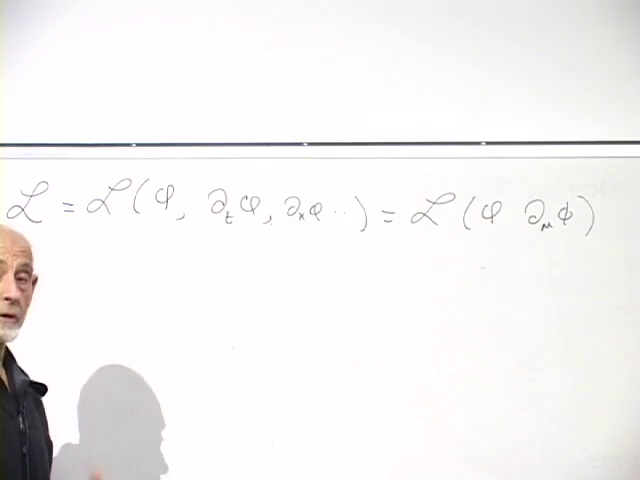
\includegraphics[width=0.82\textwidth]{lecture_09_figure_03.png}
\caption{Dépendance du lagrangien d’un champ scalaire par rapport au champ et à ses dérivées d’espace-temps.}
\lectureframe{00:03:56}
\end{figure}

L’équation d’Euler--Lagrange pour le champ est
\begin{equation}
\frac{\partial}{\partial t}
\frac{\partial\mathcal L}{\partial\dot\phi}
+
\frac{\partial}{\partial x}
\frac{\partial\mathcal L}{\partial\phi_x}
+
\frac{\partial}{\partial y}
\frac{\partial\mathcal L}{\partial\phi_y}
+
\frac{\partial}{\partial z}
\frac{\partial\mathcal L}{\partial\phi_z}
=
\frac{\partial\mathcal L}{\partial\phi},
\end{equation}
où
\begin{equation}
\dot\phi=\frac{\partial\phi}{\partial t},
\qquad
\phi_x=\frac{\partial\phi}{\partial x},
\qquad
\phi_y=\frac{\partial\phi}{\partial y},
\qquad
\phi_z=\frac{\partial\phi}{\partial z}.
\end{equation}
Si \(\mathcal L\) contient plusieurs champs, on applique cette règle séparément à chacun d’eux. On obtient ainsi le système des équations du mouvement.

L’exemple scalaire le plus simple est
\begin{equation}
\begin{split}
\mathcal L
&=
\frac12\dot\phi^2
-\frac12\phi_x^2
-\frac12\phi_y^2
-\frac12\phi_z^2
-V(\phi)
\\
&=
\frac12\dot\phi^2-\frac12(\boldsymbol\nabla\phi)^2-V(\phi).
\end{split}
\end{equation}
Les termes en dérivées spatiales ont un signe opposé à celui du terme en dérivée temporelle. En dérivant terme à terme, on obtient
\begin{align}
\frac{\partial\mathcal L}{\partial\dot\phi}&=\dot\phi,
&
\frac{\partial\mathcal L}{\partial\phi_i}&=-\phi_i,
&
\frac{\partial\mathcal L}{\partial\phi}&=-V'(\phi),
\end{align}
et donc
\begin{equation}
\ddot\phi-\nabla^2\phi=-V'(\phi).
\end{equation}

\begin{figure}[htbp]
\centering
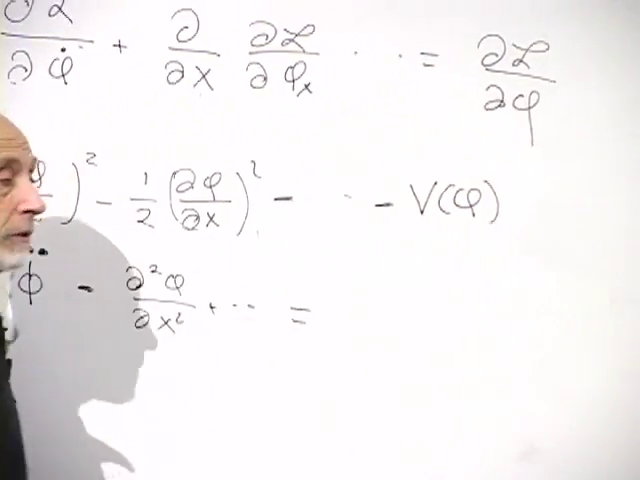
\includegraphics[width=0.74\textwidth]{lecture_09_figure_04.png}
\caption{Équation d’Euler--Lagrange, lagrangien du champ scalaire et équation de champ engendrée par \(V(\phi)\).}
\lectureframe{00:08:23}
\end{figure}

C’est l’équation engendrée par le lagrangien scalaire.\editorialnote{Le cadre conservé est tronqué sur son bord gauche ; la fin affichée est fixée par la dérivation orale qui l’entoure immédiatement.}

Ici, \(V(\phi)\) est la densité d’énergie potentielle du champ. Une contribution constante à \(V\) n’a aucun effet sur cette équation, car sa dérivée s’annule. Un potentiel linéaire est algébriquement possible, mais il n’est pas borné inférieurement : l’énergie du champ peut tendre vers moins l’infini. Le premier exemple stable est donc
\begin{equation}
V(\phi)=\frac12m^2\phi^2,
\qquad
V'(\phi)=m^2\phi,
\end{equation}
ce qui donne
\begin{equation}
\ddot\phi-\nabla^2\phi=-m^2\phi.
\end{equation}

Pour mettre en évidence la signification de \(m\), introduisons une onde plane,
\begin{equation}
\phi(\mathbf x,t)=\phi_0e^{i\omega t-i\mathbf k\cdot\mathbf x}.
\end{equation}
Alors
\begin{equation}
\ddot\phi=-\omega^2\phi,
\qquad
\nabla^2\phi=-\mathbf k^2\phi,
\end{equation}
et l’équation d’onde devient
\begin{equation}
-\omega^2\phi+\mathbf k^2\phi=-m^2\phi.
\end{equation}
Après simplification par \(\phi\),
\begin{equation}
\omega^2=\mathbf k^2+m^2.
\end{equation}
Dans le système d’unités où \(\hbar=c=1\), la fréquence correspond à l’énergie et le nombre d’onde à la quantité de mouvement. Ainsi,
\begin{equation}
E^2=\mathbf p^2+m^2,
\end{equation}
ou, en rétablissant les puissances de \(c\), \(E^2=\mathbf p^2c^2+m^2c^4\). Le paramètre \(m\) est la masse d’un quantum du champ.

L’invariance relativiste peut être imposée au niveau de l’expression compacte. Si \(\mathcal L\) est un scalaire de Lorentz, ses équations du mouvement sont invariantes de Lorentz. Le signe relatif entre les dérivées temporelles et spatiales est le signe d’espace-temps familier de la relativité restreinte.

\section{Non-linéarité et champs classiques couplés}

Les puissances supérieures d’un champ introduisent un nouveau type de comportement. Si
\begin{equation}
V(\phi)=\frac12m^2\phi^2+g\phi^3,
\end{equation}
alors
\begin{equation}
\ddot\phi-\nabla^2\phi=-m^2\phi-3g\phi^2.
\end{equation}
Les termes quadratiques du lagrangien donnent des équations linéaires en le champ. Les termes cubiques et de degrés supérieurs donnent des équations non linéaires.

Cette distinction se voit dans le mouvement des paquets d’ondes. Pour une équation linéaire, on peut additionner un paquet se propageant vers la droite et un autre se propageant vers la gauche pour former une nouvelle solution. Ils se chevauchent et interfèrent pendant un temps, puis se traversent et ressortent avec leur forme initiale. En présence de termes non linéaires, les paquets agissent les uns sur les autres. Ils peuvent se diffuser, se déformer ou se décomposer en ondes plus complexes. L’interférence temporaire d’ondes linéaires n’est pas une interaction ; une modification durable des paquets signale une non-linéarité.

Le même schéma apparaît avec deux champs scalaires. Posons
\begin{align}
\mathcal L
&=
\frac12(\partial_\mu\phi)(\partial^\mu\phi)
+\frac12(\partial_\mu\rho)(\partial^\mu\rho)
-V(\phi,\rho),
\\
V(\phi,\rho)
&=
\frac12m^2\phi^2+\frac12M^2\rho^2+\rho\phi^2.
\end{align}
Sans le dernier terme, les deux équations sont indépendantes :
\begin{equation}
\ddot\phi-\nabla^2\phi=-m^2\phi,
\qquad
\ddot\rho-\nabla^2\rho=-M^2\rho.
\end{equation}
Elles décrivent les quanta de deux espèces, de masses \(m\) et \(M\). Si l’on inclut le terme mixte,
\begin{align}
\ddot\phi-\nabla^2\phi&=-m^2\phi-2\rho\phi,
\\
\ddot\rho-\nabla^2\rho&=-M^2\rho-\phi^2.
\end{align}
chaque équation contient désormais l’autre champ. Les équations sont couplées et non linéaires : un paquet \(\phi\) diffuse un paquet \(\rho\), et réciproquement. Les termes dérivés régissent la relation énergie--quantité de mouvement, les termes quadratiques sans dérivées fixent les masses, et le terme mixte d’ordre supérieur encode l’interaction. C’est le schéma classique de base.

\section{Champs de Dirac et couplage scalaire}

Pour un champ de Dirac, l’équation est du premier ordre en temps. En notation abrégée à une dimension, l’extension aux trois directions spatiales étant sous-entendue, la structure des termes est
\begin{equation}
i\dot\Psi
\simeq
i\alpha\frac{\partial\Psi}{\partial x}+m\beta\Psi,
\qquad
i\boldsymbol\alpha\cdot\boldsymbol\nabla\Psi
=i\sum_i\alpha_i\frac{\partial\Psi}{\partial x_i}.
\end{equation}
Les matrices \(\alpha_i\) et \(\beta\) agissent sur les composantes de \(\Psi\). Un lagrangien correspondant contient un terme linéaire en \(\partial_t\Psi\), un terme bilinéaire avec dérivée spatiale faisant intervenir \(\alpha_i\), et le terme de masse bilinéaire \(m\Psi^\dagger\beta\Psi\). Seul ce fait structurel est nécessaire ici.\editorialnote{Dans le lagrangien de Dirac proposé, les signes, les parenthèses et la position de \(i\) sont explicitement laissés indéterminés dans la source. On n’en déduit aucune formule exacte dépendant des conventions.}

\begin{figure}[htbp]
\centering
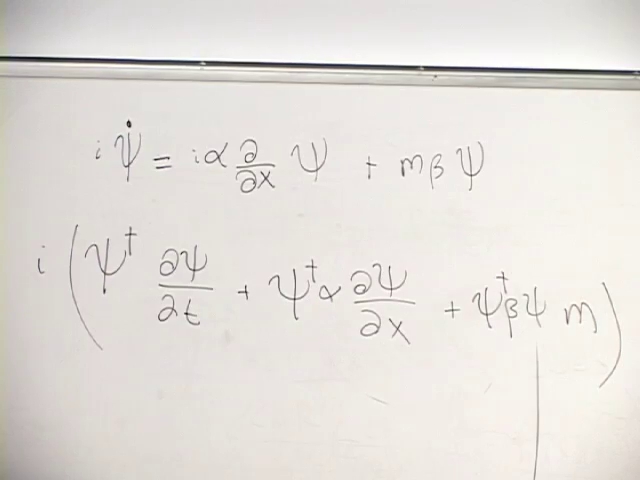
\includegraphics[width=0.76\textwidth]{lecture_09_figure_05.png}
\caption{Termes en dérivée temporelle, en dérivée spatiale et de masse dans la discussion du champ de Dirac.}
\lectureframe{00:25:37}
\end{figure}

\begin{classroomqa}
\lecturetimestamp{00:26:37}
\audiencequestion{La parenthèse du lagrangien de Dirac proposé est-elle correctement placée, avec \(i\) devant l’expression entière ?}
\lecturerresponse{Sa position n’est pas fixée ici avec certitude et n’est pas nécessaire pour établir le point structurel : il existe un lagrangien qui engendre l’équation de Dirac.}
\end{classroomqa}

Ajoutons maintenant un champ scalaire \(\phi\). Le produit naïf \(\Psi^\dagger\Psi\,\phi\) n’est pas un scalaire de Lorentz. En insérant la même matrice de Dirac que dans le terme de masse, on obtient
\begin{equation}
\mathcal L_{\mathrm{int}}
\propto
\Psi^\dagger\beta\Psi\,\phi.
\end{equation}
De façon équivalente, \(\Psi^\dagger\beta\Psi\) est le bilinéaire scalaire de Dirac. La variation du lagrangien complet ajoute à l’équation de Dirac un terme proportionnel à \(\phi\) et à l’équation scalaire une source proportionnelle à \(\Psi^\dagger\beta\Psi\). Les deux champs diffusent l’un sur l’autre.

\begin{classroomqa}
\lecturetimestamp{00:28:03}
\audiencequestion{Le \(\beta\) inséré dans l’interaction scalaire--fermionique est-il le même \(\beta\) que celui du terme de masse de Dirac ?}
\lecturerresponse{Oui. C’est la même matrice de Dirac.}
\end{classroomqa}

La comparaison
\begin{equation}
m\Psi^\dagger\beta\Psi
\qquad\hbox{and}\qquad
\Psi^\dagger\beta\Psi\,\phi
\end{equation}
fait apparaître le couplage comme un paramètre de masse remplacé par un champ scalaire. Cette observation reviendra lorsqu’on examinera, vers la fin, un champ ayant une valeur de vide non nulle.

Jusqu’ici, l’interprétation était classique : des paquets d’ondes diffusent d’autres paquets d’ondes. La même algèbre acquiert un sens particulaire plus précis lorsque les champs deviennent des opérateurs.

\section{Ce que font les puissances des champs quantiques}

Un champ quantique scalaire réel contient à la fois des opérateurs de création et d’annihilation. Schématiquement,
\begin{equation}
\phi(x)\sim A^+(x)+A^-(x),
\end{equation}
où \(A^+\) crée un quantum et \(A^-\) en annihile un. Par conséquent, \(\phi^3(x)\) contient quatre types de processus locaux :
\begin{equation}
\phi^3
\sim
(A^+)^3+(A^+)^2A^-+A^+(A^-)^2+(A^-)^3,
\end{equation}
où l’on omet, dans cette description schématique, les détails d’ordonnancement et les coefficients numériques. Les quatre variations du nombre de particules sont
\begin{equation}
3\longrightarrow0,
\qquad
0\longrightarrow3,
\qquad
2\longrightarrow1,
\qquad
1\longrightarrow2.
\end{equation}
Les trois facteurs de champ agissent tous au même point \(x\). Ainsi, un seul terme cubique comprend l’annihilation de trois particules, la création de trois particules, la fusion de deux quanta en un seul et la scission d’un quantum en deux. Dans une amplitude physique, les lois de conservation de l’énergie--quantité de mouvement peuvent ensuite éliminer certaines de ces interprétations locales, mais elles sont toutes présentes dans le produit d’opérateurs lui-même.

Les termes quadratiques libres jouent un rôle différent. Commençons par omettre le facteur de normalisation de la différence entre les points voisins \(x\) et \(x'\) :
\begin{equation}
\partial_x\phi
\ \propto\
\phi(x)-\phi(x').
\end{equation}
En élevant au carré et en développant, on obtient la structure des termes
\begin{align}
\frac12(\partial_x\phi)^2
&\ \propto\
\frac12\bigl[\phi(x)-\phi(x')\bigr]^2
\\
&=
\frac12\phi(x)^2
+\frac12\phi(x')^2
-\phi(x)\phi(x').
\end{align}
Chaque carré en un même point admet plusieurs interprétations en opérateurs : il peut créer deux quanta, en annihiler deux, ou en annihiler puis en recréer un au même point. Ces termes ne transportent pas de particule. Le terme croisé peut annihiler un quantum en \(x'\) et le créer en \(x\), ou faire l’inverse. Il agit donc comme un terme de saut entre plus proches voisins. Des facteurs répétés transportent une particule de \(x\) à \(x'\), puis à \(x''\), et ainsi de suite. Les termes quadratiques en dérivées régissent la propagation libre ; les termes cubiques et de degré supérieur diffusent, créent et annihilent des particules.

\begin{classroomqa}
\lecturetimestamp{00:36:07}
\audiencequestion{La représentation de la dérivée par une différence finie doit-elle inclure l’écart \(x-x'\) ?}
\lecturerresponse{Oui. Si l’on note l’écart \(L\), le carré de la différence fait apparaître le facteur \(L^{-2}\). Ce facteur numérique modifie le coefficient, mais pas l’interprétation en termes de saut.}
\end{classroomqa}

En rétablissant l’écart, on obtient
\begin{align}
\frac12(\partial_x\phi)^2
&\longrightarrow
\frac{1}{2L^2}\bigl[\phi(x)-\phi(x')\bigr]^2
\\
&=
\frac{1}{2L^2}\phi(x)^2
+\frac{1}{2L^2}\phi(x')^2
-\frac{1}{L^2}\phi(x)\phi(x').
\end{align}

Le terme de masse est lui aussi quadratique, mais ne contient aucune dérivée :
\begin{equation}
\frac12m^2\phi(x)^2.
\end{equation}
Dans son interprétation à une particule, un quantum incident est absorbé puis réémis au même point. Il ne se déplace pas ; ce terme pondère, ou, en ce sens, dénombre sa présence en ce point. Le même carré d’opérateurs contient aussi ses interprétations avec création de deux quanta et annihilation de deux quanta. La distinction pertinente pour le mouvement oppose donc un terme croisé reliant des points voisins à une insertion de masse agissant en un seul point.

\section{Le vertex local de l’électrodynamique quantique}

Ces schémas élémentaires de processus particulaires sont les prémices des diagrammes de Feynman. L’exemple central est l’électrodynamique quantique, théorie des électrons, des positrons et des photons.

L’équation de Dirac possède des modes d’énergie positive et négative. Dans l’ancienne terminologie, \(\Psi\) contient des opérateurs d’annihilation pour les deux types de modes, tandis que \(\Psi^\dagger\) contient les opérateurs de création correspondants. La suppression d’un électron d’énergie négative est réinterprétée comme la création d’un positron d’énergie positive. Après ce changement d’étiquettes, la décomposition schématique utile est
\begin{align}
\Psi
&\sim
C^-_{e^-}+C^+_{e^+},
\\
\Psi^\dagger
&\sim
C^+_{e^-}+C^-_{e^+}.
\end{align}
Ainsi, \(\Psi\) annihile un électron ou crée un positron, tandis que \(\Psi^\dagger\) crée un électron ou annihile un positron. Cette abréviation ne comprend aucun facteur de normalisation, indice de spin ni intégrale sur la quantité de mouvement.

L’interaction de l’électrodynamique quantique couple le courant de Dirac au quadripotentiel électromagnétique. Dans la notation par composantes utilisée ici, sa structure est
\begin{equation}
\mathcal L_{\mathrm{QED,int}}
\sim
e\left(
\Psi^\dagger\Psi\,A_0
+
\Psi^\dagger\boldsymbol{\alpha}\Psi\mathbin{\boldsymbol{\cdot}}\mathbf A
\right),
\end{equation}
où
\begin{equation}
J^0=\Psi^\dagger\Psi,
\qquad
\mathbf J=\Psi^\dagger\boldsymbol{\alpha}\Psi.
\end{equation}
Le symbole \(\sim\) est important : le signe relatif entre les termes temporel et spatial dépend des conventions adoptées pour la métrique et le potentiel vecteur. L’énoncé invariant est que le quadrivecteur courant est contracté avec le quadripotentiel.\editorialnote{La source fixe les composantes temporelle et spatiales du courant, mais ne précise pas de convention métrique pour la contraction des composantes.}

Le champ photonique \(A_\mu\) contient lui-même des opérateurs de création et d’annihilation de photons. Son caractère vectoriel porte aussi l’information sur la polarisation du photon---un petit ``repère''directionnel en plus de sa quantité de mouvement.

\begin{classroomqa}
\lecturetimestamp{00:44:28}
\audiencequestion{Comment l’interaction peut-elle être un scalaire alors que \(A_\mu\) est un vecteur et que le facteur fermionique semble d’abord être un scalaire ?}
\lecturerresponse{Les fermions fournissent eux aussi un quadrivecteur : \(\Psi^\dagger\Psi\) en est la composante temporelle et \(\Psi^\dagger\boldsymbol\alpha\Psi\) la composante spatiale. La contraction de ce courant avec \(A_\mu\) produit un scalaire.}
\end{classroomqa}

La multiplication des contenus opératoriels de \(\Psi^\dagger\), \(\Psi\) et \(A_\mu\) donne quatre interprétations familières d’un même vertex local :
\begin{enumerate}
\item un électron émet un photon ;
\item un électron absorbe un photon ;
\item un électron et un positron s’annihilent en un photon ;
\item un photon crée une paire électron--positron.
\end{enumerate}
Dans la première interprétation, \(\Psi\) annihile l’électron incident, \(\Psi^\dagger\) crée l’électron sortant, et le champ photonique crée le photon. En choisissant la partie d’annihilation du photon, on obtient l’absorption. Les composantes associées aux positrons donnent l’annihilation ou la création de paires. Un terme local contient toute cette famille de processus.

Dans un diagramme avec flux fermionique, la flèche d’une ligne de positron pointe dans le sens opposé à la propagation du positron. Avec cette convention, la flèche fermionique traverse sans interruption chaque vertex autorisé de l’électrodynamique quantique. Les quatre interprétations diffèrent par le déplacement des lignes externes entre les côtés entrant et sortant, et non par une rupture de la ligne de flux fermionique.

Toutes ces interprétations ont le même coefficient \(e\), qui est la charge électrique dans la convention microscopique utilisée. Ce coefficient est la charge électrique \(e\), et non la constante de structure fine, même si les deux sont étroitement liées. L’amplitude du vertex est proportionnelle à \(e\) ; une fois pris en compte tous les facteurs cinématiques et de normalisation, l’échelle de probabilité correspondante est proportionnelle à \(e^2\).

\begin{classroomqa}
\lecturetimestamp{00:49:44}
\audiencequestion{L’interprétation photon vers électron--positron a-t-elle le même coefficient que les autres interprétations du vertex ?}
\lecturerresponse{Oui. Elle porte le même coefficient de charge électrique \(e\).}
\end{classroomqa}

\begin{classroomqa}
\lecturetimestamp{00:49:59}
\audiencequestion{Faut-il un facteur d’échelle, puisqu’une probabilité n’a pas d’unité ?}
\lecturerresponse{Dans la convention microscopique naturelle utilisée ici, la charge \(e\) est sans dimension. Elle fixe l’échelle de l’amplitude, tandis que son carré fixe celle de la probabilité.}
\end{classroomqa}

Prenons un exemple concret : un électron frappe une paroi et s’arrête brusquement. Il existe une certaine probabilité que de l’énergie et de la quantité de mouvement soient emportées par un photon. Le facteur électromagnétique élémentaire dans l’amplitude de ce rayonnement est \(e\) ; l’échelle de probabilité contient donc \(e^2\). Cet énoncé isole le facteur de couplage ; la probabilité réelle dépend aussi de l’état de l’électron et de la cinématique.

\begin{figure}[htbp]
\centering
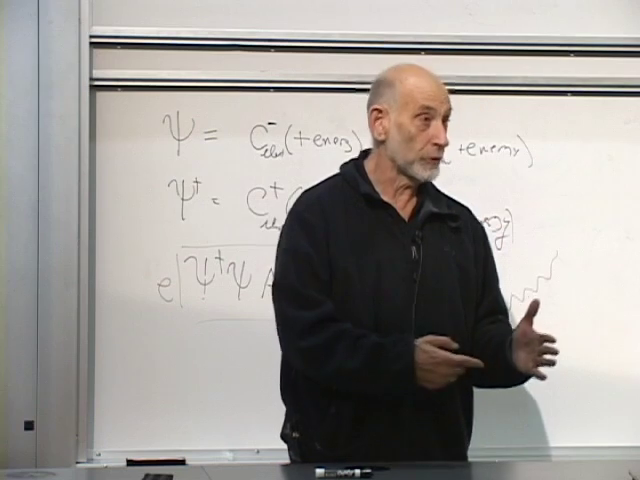
\includegraphics[width=0.78\textwidth]{lecture_09_figure_06.png}
\caption{Contenu en opérateurs d’électrons et de positrons de \(\Psi\) et \(\Psi^\dagger\), avec un schéma d’interaction électron--photon.}
\lectureframe{00:50:39}
\end{figure}

\begin{classroomqa}
\lecturetimestamp{00:51:15}
\audiencequestion{La charge électrique a-t-elle des unités ?}
\lecturerresponse{Pas dans la convention microscopique naturelle utilisée ici. La charge macroscopique est souvent exprimée en coulombs, mais la théorie des particules mesure la charge par rapport à une unité élémentaire choisie. Dans les unités de Planck ou d’autres unités naturelles, les grandeurs s’expriment par des nombres purs.}
\end{classroomqa}

La différence tient aux conventions et aux échelles. Le coulomb convient pour décrire le courant dans les fils ; un couplage sans dimension convient pour les amplitudes microscopiques.\editorialnote{Une brève question de 00:52:37--00:53:15 concernant le ``regroupement'' des termes porteurs de charge est fortement altérée et n’a donné lieu à aucune formulation précise.}

Les trois champs de l’interaction élémentaire de l’électrodynamique quantique sont évalués en un même point d’espace-temps. Aucun délai temporel interne n’est attribué au vertex lui-même.

\begin{classroomqa}
\lecturetimestamp{00:53:19}
\audiencequestion{L’absorption et la réémission de l’électron ainsi que l’émission du photon sont-elles simultanées, ou l’équation prévoit-elle un délai ?}
\lecturerresponse{Au vertex élémentaire, tous les opérateurs sont évalués au même point d’espace-temps. Le processus de base ne comporte donc aucun délai entre ces actions.}
\end{classroomqa}

\begin{classroomqa}
\lecturetimestamp{00:53:57}
\audiencequestion{Chaque grandeur conservée doit-elle être conservée séparément ?}
\lecturerresponse{Oui. La charge électrique est l’une des grandeurs qui doivent être conservées séparément.}
\end{classroomqa}

La conservation de la charge apparaît à la fois dans le diagramme et dans l’algèbre. Un processus qui transformerait un électron incident en positron sortant inverserait la charge et ne constitue pas un vertex autorisé de l’électrodynamique quantique. Lorsque le temps est représenté vers le haut, la flèche d’un électron pointe vers le haut et celle d’un positron vers le bas ; le vertex valide comporte toujours une flèche fermionique continue. Algébriquement, l’interaction contient un \(\Psi\) et un \(\Psi^\dagger\). Le premier augmente la charge d’une unité lorsqu’il annihile un électron ou crée un positron, et le second la diminue d’une unité. Leurs effets se compensent.

\begin{classroomqa}
\lecturetimestamp{00:56:05}
\audiencequestion{L’expression électron--photon encadrée est-elle le lagrangien complet de l’électrodynamique quantique ?}
\lecturerresponse{Non. C’est le terme d’interaction. Les termes quadratiques du photon libre et les termes quadratiques de Dirac, qui régissent la propagation, ne sont pas écrits.}
\end{classroomqa}

\begin{classroomqa}
\lecturetimestamp{00:56:35}
\audiencequestion{Déduit-on le lagrangien classique, tandis que le lagrangien quantique est conjecturé puis testé, et la structure énergie cinétique moins énergie potentielle subsiste-t-elle en mécanique quantique ?}
\lecturerresponse{La structure énergie cinétique moins énergie potentielle subsiste : les dérivées temporelles fournissent la forme cinétique, les gradients spatiaux la généralisent, et les termes en champs sans dérivées fournissent la forme potentielle. Le lagrangien quantique est la description la plus fondamentale. Dans un état contenant un très grand nombre de quanta, le même lagrangien produit les équations d’onde classiques. On propose des lagrangiens candidats à partir de principes physiques et de théories plus profondes, puis les expériences de collision les valident ou les réfutent.}
\end{classroomqa}

La limite des grandes occupations explique comment une même expression peut régir une théorie quantique des particules et ses ondes classiques. Cet accord n’est pas un miracle distinct imposé après coup : le champ classique est le comportement collectif d’un grand nombre de quanta. Inversement, les collisions expérimentales révèlent assez directement les vertex élémentaires pour permettre de déterminer avec une grande précision les interactions de l’électrodynamique quantique et du Modèle standard.

\section{Croisement et lois de conservation dans l’espace-temps}

Les lignes d’un vertex local peuvent être permutées entre les positions entrantes et sortantes. Une particule sortante déplacée du côté entrant est réinterprétée comme son antiparticule, et réciproquement. En ce sens, le même opérateur électron--positron--photon admet des interprétations locales en émission, en absorption, en annihilation de paires, en création de paires, et même avec toutes les particules entrantes.

\begin{classroomqa}
\lecturetimestamp{00:59:34}
\audiencequestion{Si l’on fait pivoter le diagramme d’un vertex élémentaire, reste-t-il une interprétation locale valide ?}
\lecturerresponse{Oui. On peut déplacer ses lignes externes entre les positions entrantes et sortantes, avec la réinterprétation correspondante en particule--antiparticule.}
\end{classroomqa}

L’interprétation locale de l’opérateur ne constitue pas encore un processus physique complet. Son amplitude doit être intégrée sur tous les points d’espace-temps où le vertex pourrait se produire. L’intégrale temporelle impose la conservation de l’énergie et l’intégrale spatiale celle de la quantité de mouvement. Une image où un électron, un positron et un photon disparaissent tous dans le vide figure parmi les interprétations locales formelles, mais l’amplitude intégrée s’annule, car ce processus ne peut conserver l’énergie et la quantité de mouvement.

\begin{classroomqa}
\lecturetimestamp{01:00:30}
\audiencequestion{L’image où toutes les particules sont entrantes signifie-t-elle qu’un électron, un positron et un photon peuvent disparaître dans le néant ?}
\lecturerresponse{C’est une interprétation de l’opérateur local, mais l’amplitude physique comprend une intégration sur la position du vertex. Ces intégrales imposent la conservation de l’énergie et de la quantité de mouvement ; ce processus cinématiquement interdit a donc une amplitude nulle.}
\end{classroomqa}

\begin{classroomqa}
\lecturetimestamp{01:01:57}
\audiencequestion{Existe-t-il aussi une interprétation inverse, du vide vers un électron--positron--photon, et les processus exclus disparaissent-ils après intégration ?}
\lecturerresponse{L’interprétation locale inverse est également présente. L’intégration sur l’espace et le temps élimine tout processus incompatible avec les lois de conservation.}
\end{classroomqa}

Les dérivées du lagrangien s’accordent avec le développement des opérateurs sans dériver les symboles de création et d’annihilation eux-mêmes. Un champ a schématiquement la forme
\begin{equation}
\Psi(x)
\sim
\int d^3k\,
\bigl[
C(\mathbf k)e^{i\mathbf k\cdot\mathbf x-i\omega t}
+\cdots
\bigr].
\end{equation}
Les opérateurs \(C(\mathbf k)\) sont des coefficients de ce développement en espace-temps. Les dérivées agissent sur les ondes planes et font apparaître \(\mathbf k\) ou \(\omega\).

\begin{classroomqa}
\lecturetimestamp{01:02:27}
\audiencequestion{Lorsqu’on dérive un développement de champ, l’opérateur de création lui-même est-il dérivé ?}
\lecturerresponse{Non. Dans ce développement, les opérateurs de création et d’annihilation sont indépendants de la coordonnée d’espace-temps. Les dérivées agissent sur les facteurs exponentiels et font apparaître la quantité de mouvement et la fréquence.}
\end{classroomqa}

\section{Nucléons et pions : une théorie effective}

Le même langage peut décrire les protons, les neutrons et les pions. Les protons et les neutrons sont des fermions représentés par les champs \(\Psi_p\) et \(\Psi_n\). Pour cette discussion sur le dénombrement des interactions, on traite les champs de pions comme des champs scalaires à trois états de charge :
\begin{equation}
\pi^+,
\qquad
\pi^-,
\qquad
\pi^0.
\end{equation}
Le proton et \(\pi^+\) portent chacun une unité de charge électrique positive, le \(\pi^-\) une unité négative, et le neutron ainsi que \(\pi^0\) sont neutres. À un niveau plus profond, les pions sont des systèmes quark--antiquark, mais on peut laisser cette description interne de côté dans un premier temps.

Une liste schématique de produits de champs nucléon--pion qui conserve la charge est
\begin{equation}
\mathcal L_{N\pi}
\sim
\left\{
\Psi_p^\dagger\Psi_n\,\pi^+,\;
\Psi_n^\dagger\Psi_p\,\pi^-,\;
\Psi_p^\dagger\Psi_p\,\pi^0,\;
\Psi_n^\dagger\Psi_n\,\pi^0
\right\}.
\end{equation}
Seuls le contenu en champs et les attributions de charge sont indiqués ; les coefficients relatifs, les signes et la structure des matrices spinorielles ne sont pas fixés ici. La charge du premier champ de pion se détermine en examinant une interprétation concrète : un neutron accompagné d’un pion positif peut produire un proton, alors qu’un pion négatif à sa place transformerait une charge incidente négative en une charge sortante positive. Le terme conjugué donne le processus chargé opposé.\editorialnote{Dans la source, le signe du pion est corrigé à plusieurs reprises avant d’aboutir à la paire qui conserve la charge et qui est présentée ici ; l’ordre affiché reprend cette structure schématique finale.}

Chaque terme admet de nouveau plusieurs interprétations par croisement. Déplacer un neutron sortant du côté entrant le transforme en antineutron incident. Le vertex chargé peut donc décrire la combinaison d’un proton et d’un antineutron en un \(\pi^+\), ainsi que des processus tels que \(p\to n+\pi^+\) lorsque la cinématique le permet. Les termes neutres permettent à un proton ou à un neutron d’émettre ou d’absorber un \(\pi^0\). La conservation de la charge sélectionne la famille de processus autorisée, tandis que l’énergie, la quantité de mouvement et les autres symétries déterminent lesquels peuvent se produire dans une expérience donnée.

Cette description effective était utile avant que la sous-structure des quarks soit connue. Elle reste utile lorsqu’une sonde ne peut pas résoudre cette structure. Un proton possède une distribution finie de constituants, un peu comme un atome possède une structure interne, mais à une échelle bien plus petite. Si une expérience transfère trop peu de quantité de mouvement pour briser le proton ou en résoudre la structure, on peut traiter le proton comme une particule ponctuelle dotée de son propre champ. Une collision suffisamment énergétique révèle les quarks ; le champ du proton ponctuel ne suffit alors plus.

Comme le proton est chargé, il possède aussi une interaction locale proton--photon, schématiquement \(J_p^\mu A_\mu\), où \(J_p^\mu\) est le courant du proton. L’électron possède l’interaction correspondante électron--photon. En revanche, un proton ne peut pas se transformer en neutron en émettant un photon : \(p\to n+\gamma\) ne conserve pas la charge.

\begin{classroomqa}
\lecturetimestamp{01:10:28}
\audiencequestion{Que se passe-t-il lorsqu’un proton et un électron interagissent ?}
\lecturerresponse{Chaque particule chargée possède un vertex photonique. Le proton peut émettre un photon tout en restant un proton, et l’électron peut absorber ce photon tout en restant un électron. La diffusion proton--électron s’assemble à partir de ces deux vertex locaux et de la propagation du photon entre eux.}
\end{classroomqa}

\section{Localité et répétition de processus élémentaires}

Il n’existe pas de terme non local spécial pour l’échange complet proton--électron. Un vertex local émet le photon au niveau du proton ; les termes quadratiques du photon le transportent de proche en proche, puis un autre vertex local l’absorbe au niveau de l’électron. Le processus étendu est le produit de ces éléments élémentaires.
\begin{equation}
\begin{aligned}
\bigl[J_p^\mu A_\mu\bigr](x_p)
&\longrightarrow
\underbrace{x_p\to x_1\to x_2\to\cdots\to x_e}_{\text{quadratic photon propagation}}
\\
&\longrightarrow
\bigl[J_e^\nu A_\nu\bigr](x_e).
\end{aligned}
\end{equation}
Dans cette chaîne schématique, les flèches indiquent des insertions successives entre points voisins, et non une nouvelle interaction non locale.

\begin{classroomqa}
\lecturetimestamp{01:12:06}
\audiencequestion{Comment écrirait-on le lagrangien de l’ensemble de l’échange entre le proton--l’électron ?}
\lecturerresponse{On n’ajoute pas de terme pour décrire tout le processus étendu. Celui-ci se construit à partir d’un vertex local proton--photon, de termes de propagation quadratiques répétés et d’un vertex local électron--photon.}
\end{classroomqa}

La structure locale comporte deux formes. Un terme d’interaction sans dérivée agit en un seul point de l’espace-temps. Un terme dérivé, exprimé sous forme de différence finie, ne relie ce point qu’à un point voisin. Aucun des deux types de terme ne transfère directement une particule sur une distance finie. La propagation à longue portée résulte de l’assemblage de nombreux déplacements infinitésimaux ; il n’existe pas d’action élémentaire à distance.

\begin{classroomqa}
\lecturetimestamp{01:14:36}
\audiencequestion{Le lagrangien ne contient-il des termes qu’en un seul point ?}
\lecturerresponse{Les termes d’interaction agissent en un point. Les termes dérivés relient un point à un point infiniment proche. L’émission, les nombreux sauts entre points voisins et l’absorption produisent ensemble un échange sur une distance finie.}
\end{classroomqa}

\begin{classroomqa}
\lecturetimestamp{01:15:36}
\audiencequestion{Tous les éléments du processus étendu sont-ils présents, et leur composition revient-elle à les multiplier ?}
\lecturerresponse{Oui. Chaque émission élémentaire, chaque saut ou chaque absorption est encodé dans le lagrangien. Les produits d’insertions répétées assemblent ces éléments pour former le processus de plus grande ampleur.}
\end{classroomqa}

La théorie quantique relativiste des champs considérée ici présuppose la structure de l’espace-temps sur laquelle ses champs sont définis. Il ne faut pas la confondre avec une théorie quantique complète d’une géométrie dynamique de l’espace-temps.

\begin{classroomqa}
\lecturetimestamp{01:16:28}
\audiencequestion{Cette composition reste-t-elle valable dans un régime fortement relativiste, par exemple près de l’horizon d’un trou noir ?}
\lecturerresponse{L’extension aux trous noirs sort du cadre de cette construction. La théorie quantique des champs utilisée ici ne fournit pas à elle seule une description complète de la dynamique des trous noirs, où la gravitation est essentielle.}
\end{classroomqa}

Un champ est un opérateur associé à un acte local élémentaire. Un facteur de champ peut absorber une particule ou en émettre une. Un produit de deux facteurs peut absorber une particule et en émettre une autre au même point ; des produits de degré supérieur peuvent modifier davantage le contenu en particules. Les produits d’opérateurs locaux relient ces actes pour former des histoires. Dans l’espace-temps, le mouvement se représente par l’absorption dans une petite région, la réémission dans une région voisine, une autre absorption, puis une autre réémission. Lorsque la taille du pas tend vers zéro tandis que le nombre de pas augmente, on obtient la trajectoire continue.

\begin{classroomqa}
\lecturetimestamp{01:17:30}
\audiencequestion{Comment faut-il comprendre les champs, la distance et le temps dans cette représentation par pas locaux ?}
\lecturerresponse{Les champs sont des opérateurs d’absorption et d’émission locales. Les produits combinent ces actes élémentaires, et le mouvement dans l’espace-temps se construit à partir de pas infinitésimaux entre points voisins, avant de prendre la limite continue.}
\end{classroomqa}

On peut donc partir d’une discrétisation de l’espace-temps en petites cellules, auxquelles sont associés les opérateurs de champ.\editorialnote{Les propos du public entre 01:17:30--01:20:40 sont en partie inaudibles ; la question paraphrasée ne conserve que le sujet qui peut être reconstitué, tandis que la réponse sur les opérateurs locaux et les pas successifs dans l’espace-temps est claire.} Les dérivées deviennent des différences. Les termes croisés quadratiques relient les cellules voisines, tandis que les termes de masse et d’interaction agissent à l’intérieur d’une même cellule. Les cellules servent à définir la théorie limite ; elles ne correspondent ni à des particules supplémentaires ni à une nouvelle échelle de masse physique.

Il n’est pas nécessaire d’ajouter séparément les effets de la relativité restreinte à chaque pas. Lorsque le lagrangien est un scalaire de Lorentz, les amplitudes qu’on en assemble sont invariantes de Lorentz, et des effets tels que la dilatation du temps découlent de cette structure.

\begin{classroomqa}
\lecturetimestamp{01:21:10}
\audiencequestion{Le mouvement à haute énergie et la dilatation du temps posent-ils des problèmes supplémentaires dans un processus à plusieurs étapes ?}
\lecturerresponse{Aucune correction distincte n’est nécessaire. Si le lagrangien est un scalaire de Lorentz, les effets de la relativité restreinte, comme la dilatation du temps, sont déjà intégrés au résultat. Le souci précis à l’origine de la question n’est pas tout à fait clair.}
\end{classroomqa}

Les opérateurs de création et d’annihilation peuvent être représentés dans une base de position ou dans une base d’impulsion. Un opérateur de création en espace des positions est une superposition de Fourier d’opérateurs de création en espace des impulsions, et réciproquement. Il n’existe pas d’opérateur qui crée un état dont la position et l’impulsion sont toutes deux spécifiées exactement. Localiser précisément la particule exige une large bande d’impulsions ; la localiser précisément en impulsion la délocalise en position. Dans ce langage, la relation de Fourier entre les deux bases exprime le principe d’incertitude.

\begin{classroomqa}
\lecturetimestamp{01:22:48}
\audiencequestion{Quel est le lien entre les opérateurs de création et d’annihilation, la position, l’impulsion et le principe d’incertitude ?}
\lecturerresponse{On peut les représenter comme des fonctions de la position ou comme des fonctions de l’impulsion. Les deux représentations sont transformées de Fourier l’une de l’autre. Un état fortement localisé en position requiert de nombreuses impulsions, tandis qu’un état fortement localisé en impulsion est étalé en position ; il n’existe pas d’opérateur de création pour des valeurs simultanément bien définies de \(x\) et \(p\).}
\end{classroomqa}

La construction en cellules peut maintenant être énoncée complètement. Étiquetons les cellules par \(n\), remplaçons une dérivée par une différence finie telle que
\begin{equation}
\partial_\mu\phi(x)
\longrightarrow
\frac{\phi_{n+\hat\mu}-\phi_n}{a},
\end{equation}
et plaçons chaque espèce de champ dans chaque cellule. Un terme croisé quadratique retire un quantum d’une cellule et le crée dans une cellule voisine. On obtient la théorie continue en faisant tendre l’espacement \(a\) vers zéro, une fois les expressions régularisées définies.
\begin{equation}
\underbrace{\phi_n\phi_{n+\hat\mu}}_{\text{hop }n\leftrightarrow n+\hat\mu},
\qquad
\underbrace{m^2\phi_n^2}_{\text{same-cell mass insertion}}.
\end{equation}

\begin{classroomqa}
\lecturetimestamp{01:25:16}
\audiencequestion{Peut-on mener à terme la subdivision de l’espace-temps en cellules ?}
\lecturerresponse{Oui. Les champs sont indexés par les cellules, les dérivées deviennent des différences finies et les termes quadratiques font sauter les particules entre cellules voisines. On retrouve le continuum lorsque la taille des cellules tend vers zéro.}
\end{classroomqa}

Les électrons sautent d’une cellule à l’autre par l’intermédiaire de leurs termes quadratiques, et les photons font de même. Lorsqu’un électron et un photon se rencontrent dans une cellule, l’interaction de l’électrodynamique quantique peut absorber puis réémettre l’électron, tout en créant ou en annihilant le photon. Le terme de masse scalaire s’interprète au sein d’une même cellule : une particule entre dans cette cellule et en ressort, avec un coefficient proportionnel à \(m^2\). Il ne produit pas de saut.

\begin{classroomqa}
\lecturetimestamp{01:28:18}
\audiencequestion{La taille des cellules est-elle liée au coefficient de masse ?}
\lecturerresponse{Non. La taille des cellules est un espacement de régularisation que l’on fait finalement tendre vers zéro ; le coefficient de masse est un paramètre indépendant du lagrangien.}
\end{classroomqa}

\begin{classroomqa}
\lecturetimestamp{01:28:43}
\audiencequestion{La multiplication des facteurs locaux constitue-t-elle une construction d’amplitude conjointe sur l’espace-temps, plutôt qu’une simple succession dans le temps ?}
\lecturerresponse{Oui. Les cellules couvrent l’espace-temps et leurs contributions locales se combinent sur toute cette grille. Le produit fournit une amplitude conjointe pour les événements locaux et les étapes de propagation requis.}
\end{classroomqa}

\section{Sources, détecteurs et dynamique entre les deux}

Un processus complet est une histoire dans l’espace-temps. Sa condition initiale est fixée par ce que prépare l’expérimentateur, et sa condition finale par ce qu’enregistrent les détecteurs. Un filament chaud qui émet un électron constitue une source simple. Un opérateur de champ au niveau du filament crée cet électron incident ; des opérateurs de champ aux positions des détecteurs décrivent son absorption finale.

\begin{classroomqa}
\lecturetimestamp{01:29:30}
\audiencequestion{Quelle est l’étape initiale d’un tel processus dans l’espace-temps ?}
\lecturerresponse{Elle est préparée aux sources. Un électron émis par un filament chaud en est un exemple simple : un opérateur de champ au niveau du filament crée l’électron, tandis que des opérateurs de champ aux détecteurs spécifient les événements d’absorption finaux.}
\end{classroomqa}

On peut aussi formuler la même construction à partir du vide. Les opérateurs de création aux sources construisent l’état incident sur le vide. Les opérateurs d’annihilation associés aux détecteurs sélectionnent l’état sortant. Ces opérateurs spécifient les conditions aux limites ; ils ne remplacent pas la dynamique dans toute la région comprise entre la source et le détecteur.

\begin{classroomqa}
\lecturetimestamp{01:31:11}
\audiencequestion{Serait-il erroné de placer la dynamique uniquement au niveau des émetteurs, au lieu de la faire intervenir dans tout le système ?}
\lecturerresponse{Oui. Partons du vide, utilisons les opérateurs de source pour préparer les particules incidentes, et les opérateurs de détecteur pour sélectionner les particules finales. Entre les deux, des insertions répétées du lagrangien agissent dans tout l’espace-temps, déplacent les particules, les créent et les annihilent.}
\end{classroomqa}

Avec suffisamment d’insertions, plusieurs particules peuvent se déplacer simultanément à travers de nombreuses cellules voisines ; des particules peuvent aussi être créées ou annihilées en cours de route. Les opérateurs initiaux indiquent ce qui entre, les opérateurs finaux ce qui est enregistré, et les opérations répétées du lagrangien fournissent tout ce qui se passe entre les deux.

\begin{classroomqa}
\lecturetimestamp{01:33:24}
\audiencequestion{Si un nombre arbitraire d’insertions du lagrangien peut avoir lieu, intègre-t-on leurs positions ?}
\lecturerresponse{Oui. On intègre leurs positions dans l’espace-temps. Les règles exactes de Feynman ne sont pas dérivées ici ; l’idée immédiate est que de simples expressions de champs locaux encodent les interactions primitives à partir desquelles s’assemble un processus complet.}
\end{classroomqa}

\section{Symétrie de phase, charge et amplitudes}

Écrire les processus primitifs dans un lagrangien rend aussi visibles leurs symétries. Considérons un changement global de phase du champ électronique,
\begin{equation}
\Psi\longrightarrow e^{i\theta}\Psi,
\qquad
\Psi^\dagger\longrightarrow e^{-i\theta}\Psi^\dagger,
\qquad
A_\mu\longrightarrow A_\mu.
\end{equation}
Un terme comportant autant de facteurs \(\Psi\) que de facteurs \(\Psi^\dagger\) reste inchangé, car les phases s’annulent. Un terme où ces nombres seraient différents acquérait une phase. L’égalité de ces nombres est la forme algébrique de la conservation de la charge.

C’est un avantage central de la description lagrangienne. Les facteurs de champ rendent visibles les processus élémentaires, leurs combinaisons révèlent les symétries, et les symétries mettent en évidence les lois de conservation. Des insertions répétées font évoluer l’état initial préparé vers l’état final sélectionné. Le résultat est une amplitude quantique. Son évaluation exacte exige les règles de Feynman, mais la structure apparaît déjà : les opérations locales se répètent à tous les ordres autorisés par les lois de conservation.

\section{Mesures de champ et commutateurs}

Les opérateurs de champ conservent leur sens habituel d’opérateurs en mécanique quantique. Leurs valeurs propres sont les résultats possibles de mesures de champ, et leurs vecteurs propres décrivent les états associés à ces valeurs. On peut sonder un champ électrique en y plaçant une particule chargée et en observant son accélération.

\begin{classroomqa}
\lecturetimestamp{01:37:06}
\audiencequestion{Les valeurs propres et vecteurs propres des opérateurs de champ jouent-ils leur rôle habituel en mécanique quantique ?}
\lecturerresponse{Oui. Les valeurs propres sont les valeurs de champ susceptibles d’être mesurées, et l’on peut sonder les champs par leurs effets sur les particules. Les commutateurs déterminent les restrictions aux mesures simultanées.}
\end{classroomqa}

L’identité triviale
\begin{equation}
[\phi(x),\phi(x)]=0
\end{equation}
ne tranche pas la question de la mesure. Il faut spécifier deux observables et leur relation dans l’espace-temps. Un champ et son impulsion conjuguée forment une paire canonique non commutative, et les opérateurs de champ en des points séparés par un intervalle de genre temps ne commutent pas nécessairement ; les champs bosoniques locaux commutent en revanche à séparation de genre espace, conformément à la localité. Le lien familier entre commutateurs et incertitude s’applique donc aussi ici, mais seulement après avoir correctement identifié la paire d’opérateurs.\editorialnote{La source affirme la non-commutation en des points distincts de manière trop générale. Cette précision préserve l’idée de la mesure tout en respectant la microcausalité des champs bosoniques locaux séparés par un intervalle de genre espace.}

\begin{classroomqa}
\lecturetimestamp{01:39:57}
\audiencequestion{Le champ électrique ou électromagnétique se mesure-t-il en volts ou en volts par mètre ?}
\lecturerresponse{Le champ électrique se mesure en volts par mètre. Les volts et les mètres ne sont pas les unités les plus utiles pour décrire les processus microscopiques des champs, qu’il est plus naturel d’organiser en termes de photons. À l’inverse, la théorie quantique des champs n’est pas l’outil utile pour décider comment arroser une maison.}
\end{classroomqa}

Les unités naturelles à une description ne sont pas forcément celles qui éclairent une autre description. Les volts et les volts par mètre conviennent aux appareils macroscopiques ; la création et l’annihilation de photons conviennent aux processus microscopiques.

\begin{classroomqa}
\lecturetimestamp{01:41:10}
\audiencequestion{L’idée centrale est-elle que les termes du lagrangien sont des éléments de base qu’on combine en processus plus vastes ?}
\lecturerresponse{Oui. Les processus élémentaires se répètent d’un point à l’autre. Chaque élément de base agit en un point de l’espace-temps ou relie des points voisins par un terme dérivé. Une propagation apparemment non locale se construit à partir de ces pas locaux ; il n’existe pas d’action élémentaire à distance.}
\end{classroomqa}

\section{Produits de processus locaux et sommes sur les trajets}

Il existe une manière heuristique et compacte de représenter la répétition des processus locaux. Découpons l’espace-temps en cellules et écrivons
\begin{equation}
\prod_x\bigl(1+\mathcal L_I(x)\bigr),
\end{equation}
où \(x\) désigne les cellules et où \(\mathcal L_I(x)\) est le lagrangien d’interaction local. Ce n’est pas la formule exacte dans le continuum. C’est un substitut combinatoire qui montre comment les produits engendrent toutes les sélections possibles d’événements locaux.

\begin{classroomqa}
\lecturetimestamp{01:42:18}
\audiencequestion{Peut-on condenser en une seule expression de nombreuses étapes de création, de propagation et de destruction ?}
\lecturerresponse{De façon heuristique, multiplions un facteur \(1+\mathcal L_I(x)\) pour chaque cellule de l’espace-temps. Le développement du produit engendre l’absence d’événement, un événement en n’importe quel point choisi, ou des événements en plusieurs points.}
\end{classroomqa}

Pour deux cellules,
\begin{align}
\bigl(1+\mathcal L_I(x)\bigr)
\bigl(1+\mathcal L_I(x')\bigr)
&=
1+\mathcal L_I(x)+\mathcal L_I(x')
\notag\\
&\quad{}+\mathcal L_I(x)\mathcal L_I(x').
\end{align}
Le premier terme signifie qu’aucune des deux interactions n’a lieu. Les deux termes suivants placent une interaction élémentaire en \(x\) ou en \(x'\). Le dernier terme place des interactions aux deux points. Avec de nombreux facteurs, on obtient des termes impliquant un point, deux points, trois points, et ainsi de suite. Un terme comportant plusieurs vertex peut décrire, par exemple, deux particules incidentes qui produisent trois particules sortantes.

Les éléments quadratiques de propagation entrent dans la même construction. Un déplacement fini se représente par une chaîne d’insertions entre points voisins. Le produit développé contient des facteurs en une cellule, dans sa voisine, dans la suivante, et ainsi de suite, qui transportent une particule entre les extrémités.

\begin{classroomqa}
\lecturetimestamp{01:46:29}
\audiencequestion{Si une propagation sur une distance finie exige de nombreux termes de mouvement locaux, comment retrouve-t-on le mouvement requis ?}
\lecturerresponse{Le grand produit contient des chaînes d’insertions entre points voisins qui transportent la particule de son point initial à son point final. Il existe généralement de nombreuses chaînes de ce type, suivant des trajets différents. Chaque trajet contribue une amplitude, et l’amplitude totale est leur somme.}
\end{classroomqa}

Si \(r\) désigne un trajet, alors, schématiquement,
\begin{equation}
\mathcal A_{\mathrm{total}}=\sum_r\mathcal A_r,
\qquad
P=\left|\mathcal A_{\mathrm{total}}\right|^2.
\end{equation}
On n’attribue pas de probabilités ordinaires aux trajets pour les additionner ensuite. On additionne d’abord les amplitudes :
\begin{equation}
\left|\sum_r\mathcal A_r\right|^2
=
\sum_r|\mathcal A_r|^2
+
\sum_{r\ne s}\mathcal A_r\mathcal A_s^*.
\end{equation}
Les termes croisés expriment l’interférence.

\begin{classroomqa}
\lecturetimestamp{01:48:27}
\audiencequestion{Est-ce cohérent avec l’expérience des deux fentes ?}
\lecturerresponse{Tout à fait. Les chemins possibles par les deux fentes contribuent des amplitudes. Élever leur somme au carré produit des termes d’interférence, tout comme interfèrent les nombreux trajets dans l’espace-temps de la construction par pas locaux.}
\end{classroomqa}

\begin{classroomqa}
\lecturetimestamp{01:49:00}
\audiencequestion{D’où vient le \(1\) dans chaque facteur \(1+\mathcal L_I\) ?}
\lecturerresponse{C’est un dispositif combinatoire qui permet à une cellule de contribuer sans interaction aussi bien qu’avec une interaction. Il est lié aux méthodes d’intégrale de chemin, mais le produit affiché n’est qu’une approximation heuristique de l’expression technique.}
\end{classroomqa}

Le formalisme exact fournit les intégrations dans l’espace-temps, l’ordonnancement, la normalisation et les phases appropriés. Le produit est utile parce qu’il révèle les combinaisons sans prétendre constituer le formalisme complet.

\begin{classroomqa}
\lecturetimestamp{01:49:57}
\audiencequestion{S’agit-il du principe de l’action stationnaire ?}
\lecturerresponse{Non. Le principe classique de l’action stationnaire sélectionne une trajectoire classique privilégiée. En mécanique quantique, on somme plutôt les amplitudes sur les trajectoires, leurs poids étant déterminés par l’action. Même un trajet extrêmement indirect---qui passe par Paris pour aller d’un bureau à une maison voisine---fait partie de la somme quantique.}
\end{classroomqa}

Le contraste est simple, même si la relation est subtile. La mécanique classique sélectionne un chemin stationnaire. La mécanique quantique somme les chemins ; dans la limite appropriée, les phases s’additionnent de façon constructive autour de la trajectoire classique.

\section{Déduire le lagrangien et choisir un secteur}

Une fois le lagrangien et le processus spécifié, les règles de calcul de sa probabilité sont déterminées. Le calcul peut néanmoins exiger de l’ingéniosité, comme c’est souvent le cas en mathématiques difficiles, mais la véritable incertitude consiste à découvrir quels champs et quels couplages la nature utilise.

\begin{classroomqa}
\lecturetimestamp{01:50:43}
\audiencequestion{L’art consiste-t-il à exprimer le lagrangien ou à l’utiliser ?}
\lecturerresponse{L’essentiel de l’art consiste à déduire le lagrangien à partir des données expérimentales. Une fois celui-ci connu, un processus tel que l’entrée de deux particules et la sortie de quatre possède une amplitude déterminée, calculable au moyen de règles précises. Effectuer les calculs mathématiques peut demander de l’ingéniosité, mais cela ne constitue pas une ambiguïté de la théorie.}
\end{classroomqa}

Les collisions de particules mettent en évidence les vertex élémentaires. On propose des termes, souvent guidé par des symétries et des principes plus profonds, puis on confronte les amplitudes obtenues aux résultats observés. La réussite de cette démarche fixe à la fois les combinaisons de champs autorisées et leurs coefficients numériques.

\begin{classroomqa}
\lecturetimestamp{01:52:24}
\audiencequestion{Existe-t-il un lagrangien distinct pour chaque interaction---un gros livre de lagrangiens ?}
\lecturerresponse{L’image de travail est plutôt celle d’un grand lagrangien qui contient tous les champs et toutes les interactions, même si cette image pourrait finalement se révéler fausse. Des secteurs reconnaissables apparaissent comme des éléments de cette somme. Une nouvelle particule ajoute un champ ; un nouveau processus primitif ajoute un terme d’interaction.}
\end{classroomqa}

L’expression complète peut être désordonnée sans pour autant remplir un livre. Pour donner un ordre de grandeur très approximatif, on peut imaginer une centaine d’objets appelés particules élémentaires et plusieurs centaines de termes. L’électrodynamique quantique, les interactions forte et faible, ainsi qu’un secteur gravitationnel pourraient encore tenir sur quelques pages très denses. Le nombre exact n’est pas l’essentiel. L’image de travail est celle d’une expression dynamique unique, assemblée à partir de nombreux éléments reconnaissables ; cette image pourrait, explicitement, se révéler incomplète à terme.

La question de savoir si les champs déterminent une géométrie de l’espace-temps plus fondamentale dépasse le cadre de la théorie quantique des champs standard utilisée ici.\editorialnote{La question posée entre 01:55:00--01:55:20 est trop endommagée pour identifier de façon fiable la variété ou la construction géométrique concernée ; seule cette réponse délimitant le champ de la discussion peut être retenue.}

\begin{classroomqa}
\lecturetimestamp{01:55:22}
\audiencequestion{Les nombres déterminés expérimentalement sont-ils les constantes de couplage ?}
\lecturerresponse{Les constantes de couplage sont les coefficients des termes du lagrangien. Le coefficient \(m^2\) d’un terme de masse quadratique en est un exemple ; les coefficients de \(\phi^4\), de \(\phi^6\) ou de puissances encore supérieures en sont d’autres.}
\end{classroomqa}

Un même coefficient contrôle une famille d’amplitudes apparentées, car chaque produit de champs admet plusieurs interprétations en termes de création et d’annihilation. Connaître le lagrangien détermine donc bien davantage qu’une seule réaction isolée.

\begin{classroomqa}
\lecturetimestamp{01:56:05}
\audiencequestion{Faut-il connaître le lagrangien entier pour calculer l’électrodynamique quantique ?}
\lecturerresponse{Une précision infinie exigerait de prendre en compte tous les secteurs par lesquels les électrons et les photons peuvent interagir. Aux énergies atomiques, toutefois, on peut normalement isoler le secteur électron--photon. L’énergie est insuffisante pour résoudre la structure infime des quarks ; on peut donc négliger les autres secteurs avec la précision requise.}
\end{classroomqa}

Les calculs pratiques utilisent le secteur pertinent à l’échelle expérimentale. Cela ressemble à l’hydrodynamique : un système microscopique complexe peut admettre une description précise à gros grains sans révéler tous ses constituants plus profonds. La théorie quantique des champs peut donc être phénoménologique et exacte à la fois---phénoménologique par les champs et les coefficients déduits des expériences, exacte par les règles appliquées une fois ces éléments spécifiés.

\begin{classroomqa}
\lecturetimestamp{01:58:09}
\audiencequestion{Le modèle standard inclut-il la gravitation, et ces lagrangiens relativistes incluent-ils la relativité générale ?}
\lecturerresponse{La théorie officiellement appelée modèle standard n’inclut pas la gravitation, même si l’on peut ajouter celle-ci lorsqu’on considère une théorie plus générale. Les théories des champs étudiées ici combinent la mécanique quantique et la relativité restreinte. Elles n’incluent pas à elles seules la relativité générale.}
\end{classroomqa}

\section{Une valeur du vide comme coefficient de masse}

La masse d’un champ scalaire apparaît comme le coefficient de \(\phi^2\). Une interaction avec un autre champ peut donc imiter un terme de masse lorsque cet autre champ possède une valeur du vide non nulle.

\begin{classroomqa}
\lecturetimestamp{01:59:16}
\audiencequestion{Si les masses des particules résultent d’interactions de Higgs, un couplage de Higgs peut-il jouer le rôle d’un terme de masse ?}
\lecturerresponse{Oui. Un terme \(H\phi^2\) est cubique et représente habituellement une interaction avec deux lignes \(\phi\) et une ligne \(H\). Si le potentiel \(V(H)\) sélectionne un vide où \(H\) est non nul, cette valeur du vide est un nombre qui multiplie \(\phi^2\) ; elle contribue donc à un terme de masse quadratique effectif.}
\end{classroomqa}

Considérons schématiquement
\begin{equation}
\mathcal L\supset H\phi^2-V(H).
\end{equation}
En tant que terme opératoriel, \(H\phi^2\) peut absorber un \(\phi\), en émettre un \(\phi\), et émettre ou absorber un quantum \(H\). Supposons que le potentiel ait deux minima situés hors de \(H=0\), et que le vide sélectionne l’un d’eux :
\begin{equation}
\langle H\rangle=v\ne0.
\end{equation}
Écrivons le champ comme la somme de sa valeur dans le vide et d’une fluctuation,
\begin{equation}
H=v+h.
\end{equation}
Alors
\begin{equation}
H\phi^2=v\phi^2+h\phi^2.
\end{equation}
Le premier terme est quadratique en \(\phi\) et contribue à son coefficient de masse ; le second reste une interaction avec le champ fluctuant \(h\).\editorialnote{La source termine la phrase en indiquant que la valeur non nulle du vide devient un coefficient de masse. La substitution affichée complète immédiatement l’algèbre ; sa normalisation et son signe dépendent des conventions retenues pour le lagrangien complet.}

\begin{classroomqa}
\lecturetimestamp{02:01:29}
\audiencequestion{Le modèle standard inclut-il la création et l’annihilation de particules virtuelles ?}
\lecturerresponse{Absolument. La création et l’annihilation virtuelles sont inhérentes aux processus quantiques répétés encodés par le lagrangien du modèle standard.}
\end{classroomqa}